\documentclass[compress]{beamer}
\usepackage[utf8]{inputenc}
\usepackage[francais]{babel}
\usepackage[T1]{fontenc}
\usepackage{amssymb}
\usepackage{amsmath}
\usepackage{amsfonts}
\usepackage{hyperref}
\usepackage[]{algorithm2e}
\usepackage{amssymb}
\usepackage{verbatim}
\usepackage{listings}
\usepackage{color}
\usepackage{graphicx}
\usetheme[navigation]{UMONS}

\author{Clément Tamines, Florent Delgrange}
\title[ ]{Time, Clocks, and the Ordering of Events in a Distributed System}

\setbeamercovered{transparent} 
\setbeamertemplate{navigation symbols}{} 
\institute{UMONS\\Faculté des Sciences\\MA1 Sciences Informatiques\\[2ex]
  
\includegraphics[height=4ex]{UMONS}\hspace{2em}%
  \raisebox{-1ex}{
\includegraphics[height=6ex]{UMONS_FS}}}
\date{novembre 2016} 
\definecolor{darkgreen}{rgb}{0.0, 0.2, 0.13}
\subject{Réseaux II} 
\begin{document}

\begin{frame}
\titlepage
\end{frame}

\begin{frame}
\tableofcontents
\end{frame}

\section{Introduction}

\begin{frame}
\frametitle{Problématiques}
Dans un système distribué, il n'est pas toujours possible de dire qu'un événement A s'est passé avant un événement B. \\ \bigskip
\begin{itemize}
\item Comment définir un ordre chronologique entre les évènements dans un système distribué ?
\item Comment définir qu'un évènement A précède un évènement B ?
\item Comment faire en sorte que cet ordre soit total ?
\item Comment assurer la fiabilité des mécanismes de synchronisation ?
\end{itemize}
\end{frame}

\begin{frame}
\frametitle{Système distribué}
	\begin{definition}
		Un système distribué consiste en un ensemble de processus séparés dans l'espace et qui communiquent entre eux via 			messages.
	\end{definition}
	\bigskip
	Exemples : 
	\bigskip
	\begin{itemize}
		\item Ordinateurs dans un réseau
		\item Plusieurs processus communiquant entre eux dans un ordinateur.
		\item Plusieurs threads d'un processeur
	\end{itemize}
\end{frame}

\begin{frame}
\frametitle{Temps physique}

Manière intuitive d'ordonner deux événements a et b :  \\ 
\begin{center}
 "a est arrivé avant b si a est arrivé plus tôt dans le temps que b"
\end{center}
Problèmes : \\
\bigskip
\begin{itemize}
\item Le temps doit être observable dans le système
\item Le système doit donc contenir des horloges 
\item Celles-ci ne sont pas parfaitement fiable et ne donnent pas assez précisément le temps physique
\end{itemize}
\bigskip
$\implies$ la relation \textit{est arrivé avant} doit s'exprimer sans horloge réelle.
\end{frame}

\section{Ordre partiel}

\begin{frame}
\frametitle{\'Evènements dans un processus}
\begin{columns}
    \begin{column}{0.2\textwidth}
    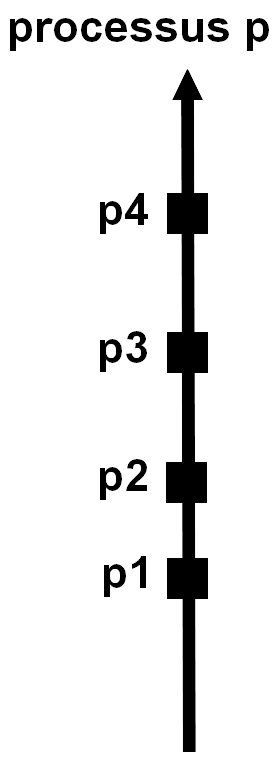
\includegraphics[scale=0.7]{clem1.png}
    \end{column}
  
    \begin{column}{0.8 \textwidth}
    \begin{itemize}
    \item Chaque processus est une suite d'événements
    \item La suite d'événements forme une séquence
    \item Dans la séquence, a se produit avant b ssi a est exécuté avant b
    \item La séquence est totalement ordonnée
    \item La réception et l'envoi de message sont des événements
    \end{itemize}
    \end{column}
\end{columns}
\end{frame}


\begin{frame}
\begin{definition}
La relation $\rightarrow$ sur un ensemble d'évènements d'un système satisfait
\begin{enumerate}
\item Si $a$ et $b$ sont deux évènements du même processus et a survient avant b, alors $a \rightarrow b$
\item Si $a$ correspond à l'envoi d'un message par un processus et b correspond à la réception de ce message par un autre processus, alors $a \rightarrow b$
\item $\rightarrow$ est transitif
\item Deux évènements $a, b$ sont concurrents ssi $a \not\rightarrow b$ et $b \not\rightarrow a$
\end{enumerate}
\end{definition}
\end{frame}

\begin{frame}
  \begin{columns}
    \begin{column}{.4\textwidth}
		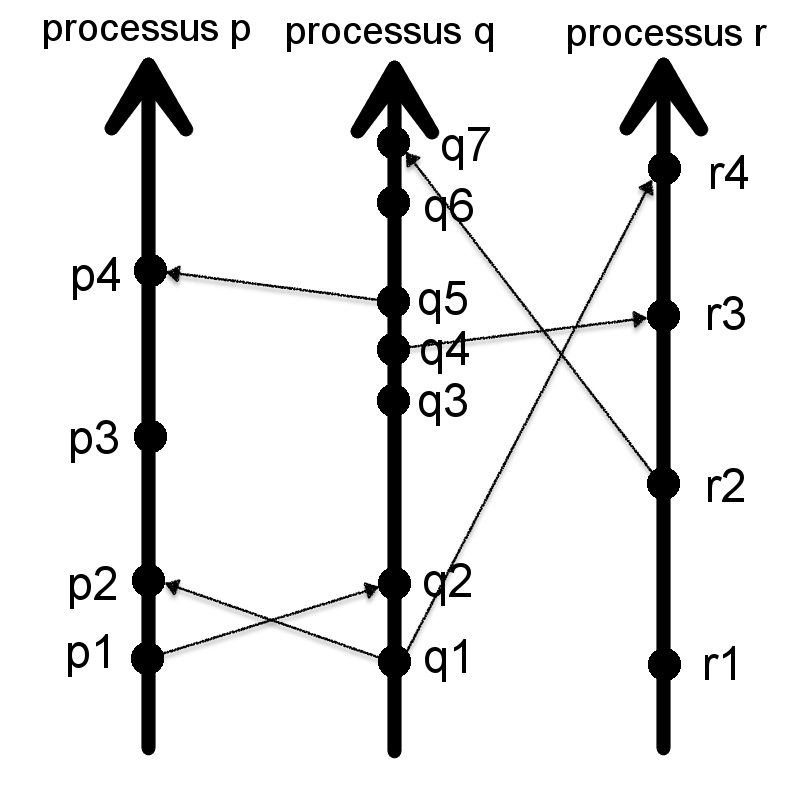
\includegraphics[scale=0.19]{process2.png}
    \end{column}
	\begin{column}{0.6 \textwidth}
\begin{center}
$p_1 \rightarrow r_4$  par transitivité avec \\
\bigskip
	$p_1 \rightarrow q_2$\\$q_2 \rightarrow q_3$ \\ $q_3 \rightarrow q_4$ \\ $q_4 \rightarrow r_3$ \\ $r_3 \rightarrow r_4$\\
\end{center}
	\end{column}
	\end{columns}
	\bigskip	\textbf{{\color{red}Problème : }}$q_3$ est concurrent avec $p3$ : on ne peut pas déterminer si $q_3$ s'est passé avant $p_3$ ou vice versa.
\end{frame}

\section{Horloges Logiques}

\begin{frame}
\frametitle{Horloges logiques}
Une horloge est une façon d'assigner un nombre à un évènement où le nombre correspond au temps où l'évènement s'est produit.\\\bigskip
$\implies$ Chaque processus $p_i$ possède une horloge $C_i$.\\
$\implies$ Une horloge $C_i$ est une fonction qui associe un nombre $C_i$<$a$>  à chaque événement $a$ dans $P_i$\\
$\implies$ Le système entier est représenté par la fonction $C$.
\begin{block}{Propriétés}
\begin{itemize}
\item Soit b, un évènement, $C$<$b$>$ = C_j$<$b$> ssi $b$ est un évènement du processus $P_j$.\\
\item $\forall i$, $C_i$ peut être simplement implémenté à l'aide de compteurs sans mécanisme lié au temps.
\end{itemize} 
\end{block}
\end{frame}

\begin{frame}
\frametitle{Conditions}
\begin{block}{Condition faible}
$a \rightarrow b \implies C$<$a$> $ < C$<$b$>
\end{block}
\bigskip
Soient $a, b$ deux événements concurrents. \\On a $a \not\rightarrow b$  et $a \not\rightarrow b$ donc\\
\begin{center}
$C$<$a$>  $\geq$ $C$<$b$> $\land$ $C$<$a$>  $\leq$ $C$<$b$>  $\implies$ $C$<$a$> = $C$<$b$>
\end{center}
Les événements $a$ et $b$ doivent être simultanés !
\end{frame}
\begin{frame}

\begin{columns}
    \begin{column}{.35\textwidth}
		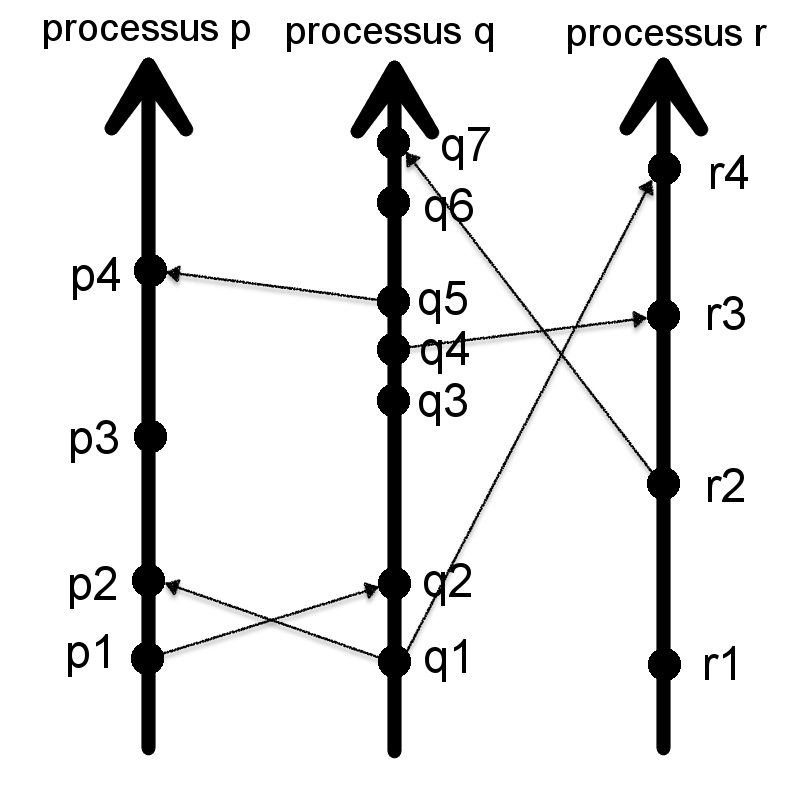
\includegraphics[scale=0.15]{process2.png}
    \end{column}
	\begin{column}{0.65 \textwidth}
\textbf{{\color{red}Problème : }}$p_2$ et $p_3$ sont concurrents de $q_3$. Donc $C$<$p_2$> = $C$<$p_3$> = $C$<$q_3$>. \\
Mais $p_2 \rightarrow p_3$ donc $C$<$p_2$> $<$ $C$<$p_3$>\\ \bigskip
$\implies$ Besoin de conditions plus fortes
	\end{column}
	\end{columns}
\begin{block}{Conditions fortes}
\begin{enumerate}
\item Si $a$ et $b$ sont des évènements de $P_i$ et que $a$ vient avant $b$, alors $C_i$<$a$> $<$ $C_i$<$b$>
\item Si $a$ est l'envoi d'un message par un processus $P_i$ et que $b$ est la réception de ce message par le processus $j$, alors $C_i$<$a$> $< C_j$<$b$>
\end{enumerate}
\end{block}
\end{frame}

%\begin{frame}
%\begin{figure}
%		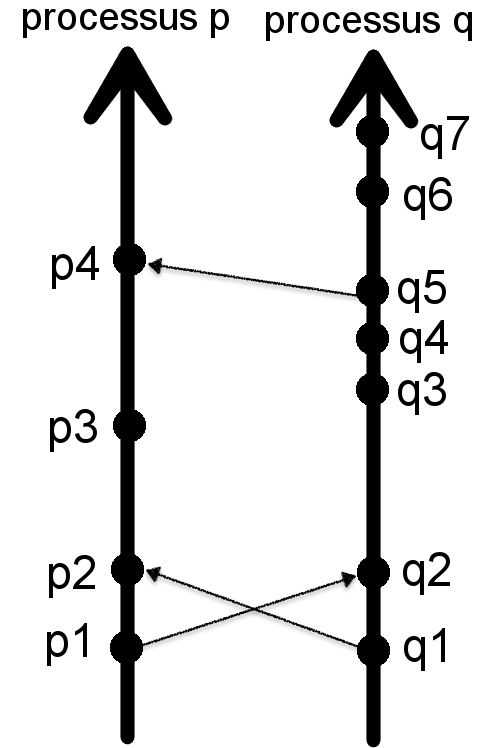
\includegraphics[scale=0.17]{process3.png}

%\end{figure}
%\textbf{Exemples : }\\
%		$C$<$p_1$> $< C$<$p_3$>\\
%		$C$<$q_5$> $< C$<$p_4$>
%\end{frame}

\begin{frame}
\frametitle{Implémentation}
\begin{block}{Condition faible}
Chaque processus $P_i$ incrémente le compteur $C_i$ entre 2 évènements successifs.\\
Soient $a$ et $b$, deux évènements successifs de $P_i$. \\
Alors après $a$, $C_i \leftarrow C_i + 1$.
\end{block}
\end{frame}

\begin{frame}
	\frametitle{Implémentation}
	\begin{block}{Condition forte}
	\begin{enumerate}[(a)]
		\item Si un évènement $a$ est l'envoi d'un message $m$ par le processus $P_i$, alors le message $m$ contient un Timestamp $T_m \leftarrow C_i$<$a$>
		\item Lorsqu'il reçoit un message $m$, le processus $P_j$ assigne la valeur $\mu$ son compteur $C_j$ tel que $\mu > T_m$ et $\mu \geq$ valeur de $C_j$ avant la réception de $m$
	\end{enumerate}
	\end{block}
	\bigskip
	L'utilisation d'un Timestamp permet au processus qui reçoit un message de mettre à jour son compteur pour que que celui-ci respecte bien la condition faible (ordre dans ce même processus) et forte (ordre entre les processus).
\end{frame}

\section{\'Evènements totalement ordonnés}
\begin{frame}
\frametitle{Ordre total}
On souhaite avoir un système d'horloge qui satisfait les conditions d'horloge précédemment énoncées et qui met en place un \textit{\textbf{ordre total}}.\\
\textbf{Rappel : }
\begin{block}{Ordre Total}
Une \textbf{relation binaire} $\preceq$ sur un ensemble E est un ordre total si $\forall x, y, z \in E$, \\
\begin{itemize}
\item \textbf{Réflexivité :} $x \preceq x$
\item \textbf{Antisymétrie :} $x \preceq y$ et $y \preceq x \implies x = y$
\item \textbf{Transitivité :} $x \preceq y$ et $y \preceq z \implies x \preceq z$
\end{itemize}
\end{block}
\end{frame}

\begin{frame}
\frametitle{Ordre Total}
Soit $\preceq$, un ordre total arbitraire sur l'ensemble des processus. On définit la relation $\Rightarrow$ comme suit :\\
Si $a \in P_i$ et $b \in P_j$, alors \\
\[
	a \Rightarrow b \ \ \text{ssi}
	\begin{cases}
		C_i \text{<}a\text{>} < C_j\text{<}b\text{>} \\
		\text{ou}\\
		C_i\text{<}a\text{>} = C_j\text{<}b\text{>} \text{ et } P_i \preceq P_j
	\end{cases}
\]
Avec une telle définition, on a bien que si $a \rightarrow b$, alors $a \Rightarrow b$. (L'ordre partiel est étendu à un ordre total)
\vspace{.5in}

\^Etre capable d'ordonner totalement les évènements peut être très utile dans l'implémentation d'un système distribué. C'est le but d'un système à horloges logiques.
\end{frame}

\begin{frame}
\frametitle{Partage de ressource}
On considère à présent un système composé d'un ensemble fini de processus qui partagent une ressource unique. On veut que les processus se synchronisent et évitent les conflits.
\begin{block}{Propriétés}
\begin{enumerate}
\item Un processus qui monopolise une ressource doit l'avoir libérée avant d'en monopoliser une autre
\item Les requêtes pour les ressources doivent être accordées dans l'ordre dans lesquelles elles ont été demandées
\item Si chaque processus qui détient une ressource la libère, alors on a que chaque requête sera accordée à un moment donné
\end{enumerate}
\end{block}
\end{frame}

\begin{frame}
Un système d'horloge centrale qui alloue des requêtes dans l'ordre dont elles sont reçues ne fonctionnera pas.\\
Soient $P_0, P_1, P_2$, des processus. On suppose que $P_1$ envoie une requête à $P_0$ et envoie ensuite
un message à $P_2$. Lorsque $P_2$ reçoit le message, $P_2$ envoie une requête à $P_0$. Il est possible que la requête de $P_2$ atteigne $P_0$ avant la requête de $P_1$.
\begin{figure}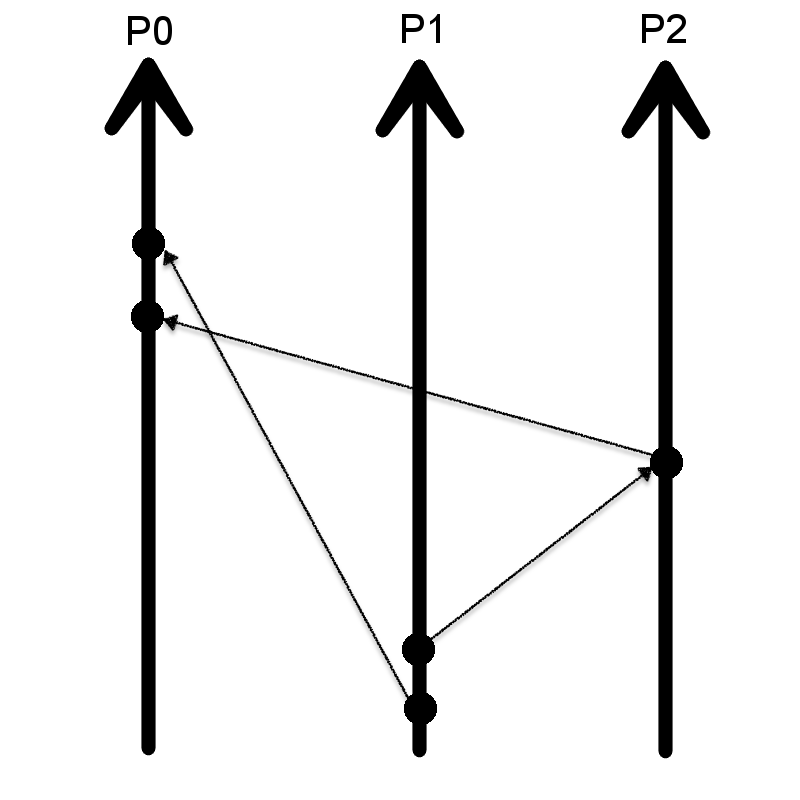
\includegraphics[scale=0.12]{process4.png}\end{figure}
La 2e condition de ce système est donc violée si la requête de $P_2$ est accordée en premier.
\end{frame}

\begin{frame}
Pour éviter ce problème : système d'horloge avec les règles {\color{cyan} IR 1} et {\color{cyan} IR 2} pour avoir un ordre total $\Rightarrow$ sur les évènements. On y rajoute les suppositions suivantes :
\begin{enumerate}
\item On suppose que pour tout processus $P_i$ et $P_j$, les messages envoyés de $P_i$ à $P_j$ sont reçus dans le même ordre qu'ils sont envoyés. \begin{figure}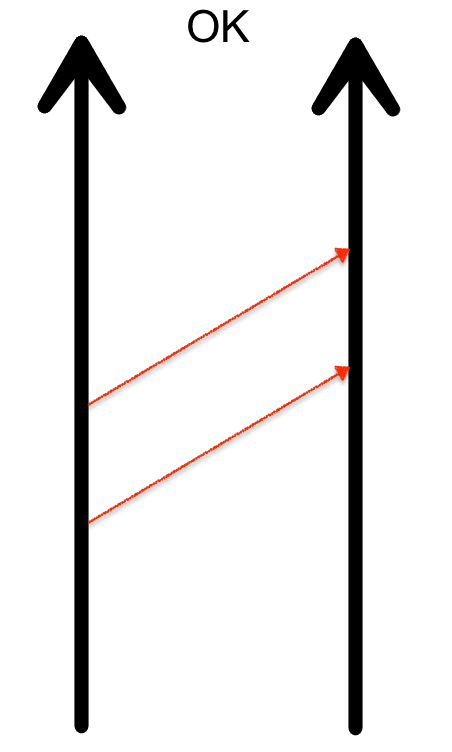
\includegraphics[scale=0.06]{process5.png}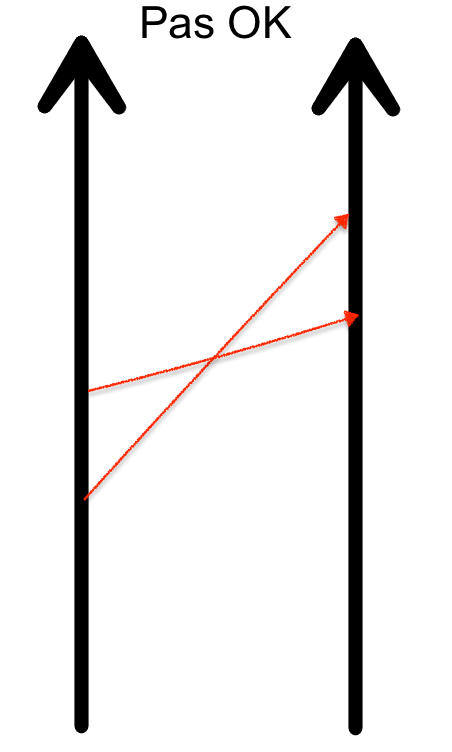
\includegraphics[scale=0.06]{process6.png}\end{figure}
\item On suppose que chaque message envoyé finit toujours par être reçu. \begin{figure}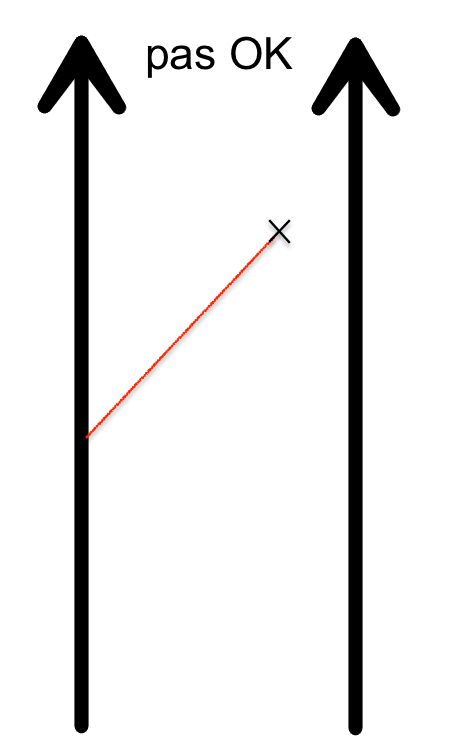
\includegraphics[scale=0.06]{process7.png}\end{figure}
\item On suppose qu'un processus peut envoyer des messages vers tout autre processus.
\end{enumerate}
Notons que les deux premières suppositions peuvent être évitées à l'aide d'un \textit{protocole d'acknowledgment} ou par numérotation des messages.
\end{frame}

\begin{frame}
\frametitle{Algorithme}
\begin{itemize}
\item Tout processus maintient une file de requête (file de priorité) invisible à tout autre processus.
\item Initialisation de la file : {$T_0:P_0$ [request resource]} avec $\forall i,  T_0 \leq C_{i_0}$ et $P_0$, le processus auquel la ressource est accordée à l'initialisation.
\end{itemize}
	\begin{columns}
    	\begin{column}{.65\textwidth}
			$P_i$ envoie une requête à la ressource sous forme d'un message contenant $T_m : P_i$ [request resource] à tous les autres processus et place ce message sur sa file de requête où $T_m$ est le timestamp de ce message.
		\end{column}
		\begin{column}{.35\textwidth}
			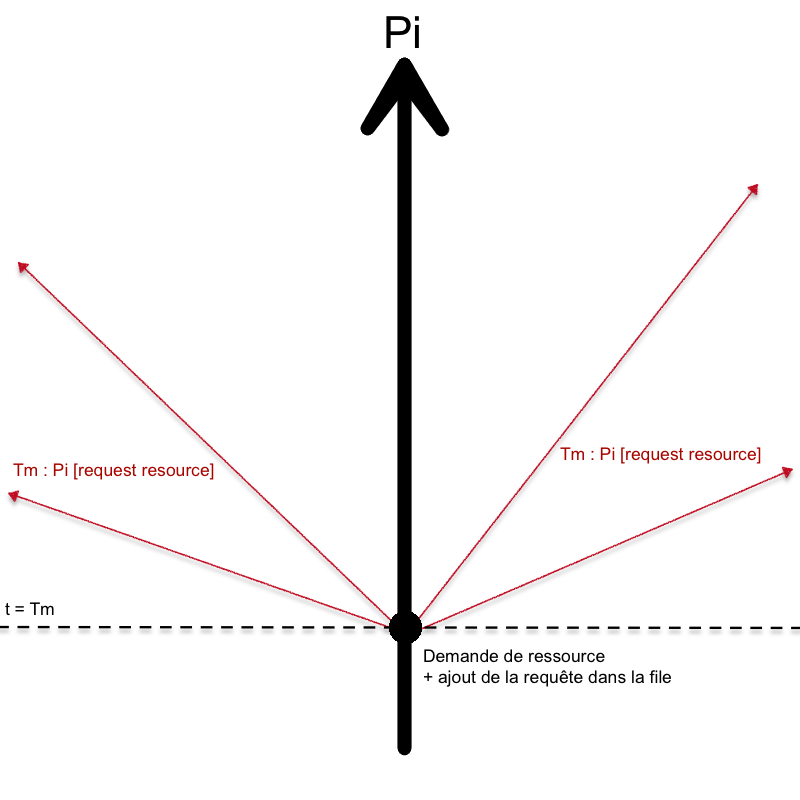
\includegraphics[scale=0.13]{process8.png}
		\end{column}
	\end{columns}
%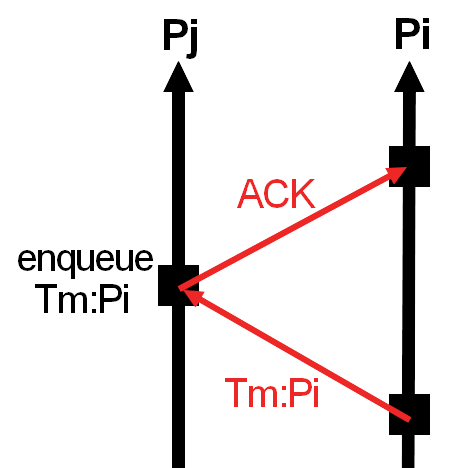
\includegraphics[scale=0.1]{process9.png}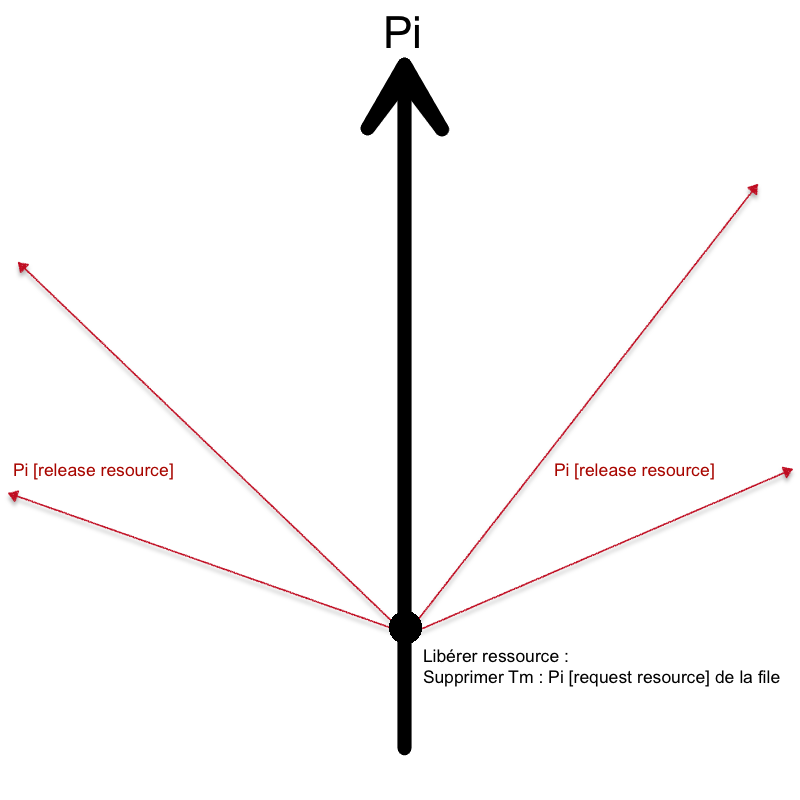
\includegraphics[scale=0.1]{process10.png}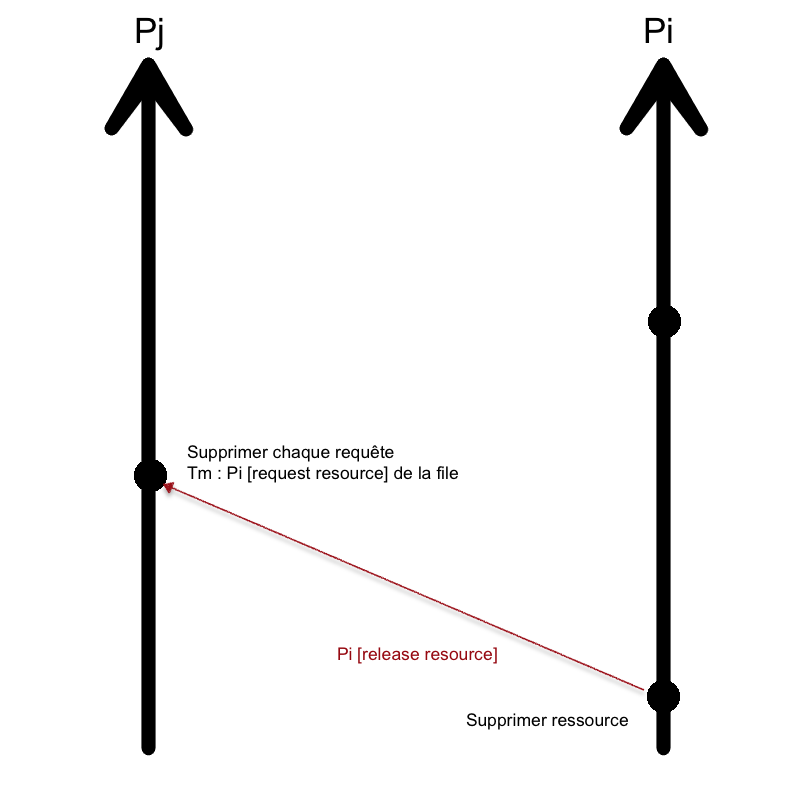
\includegraphics[scale=0.1]{process11.png}
\end{frame}

\begin{frame}
\frametitle{Algorithme}
	\begin{columns}
    	\begin{column}{.65\textwidth}
			Lorsque le processus $P_j$ reçoit le message $T_m : P_i$[request resource], celui-ci le place dans sa file de requête et envoie un acknowledgment à $P_i$ lorsque ce message se trouve à la tête de la file.
		\end{column}
		\begin{column}{.35\textwidth}
			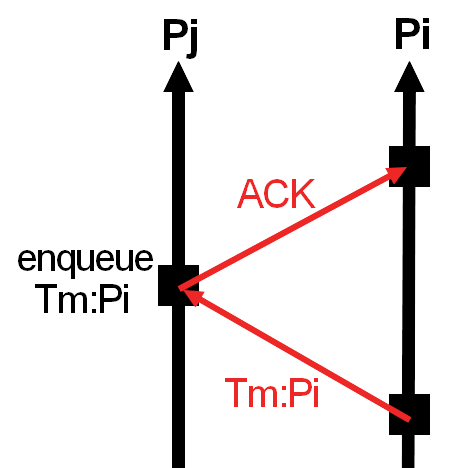
\includegraphics[scale=0.13]{process9.png}
		\end{column}
	\end{columns}
	
		\begin{columns}
    	\begin{column}{.65\textwidth}
			Pour libérer la ressource, le processus $P_i$ supprime tout $T_m : P_i$[request resource] de sa file de requête et envoie un $P_i$[release resource] sous forme de message à chaque autre processus.
		\end{column}
		\begin{column}{.35\textwidth}
			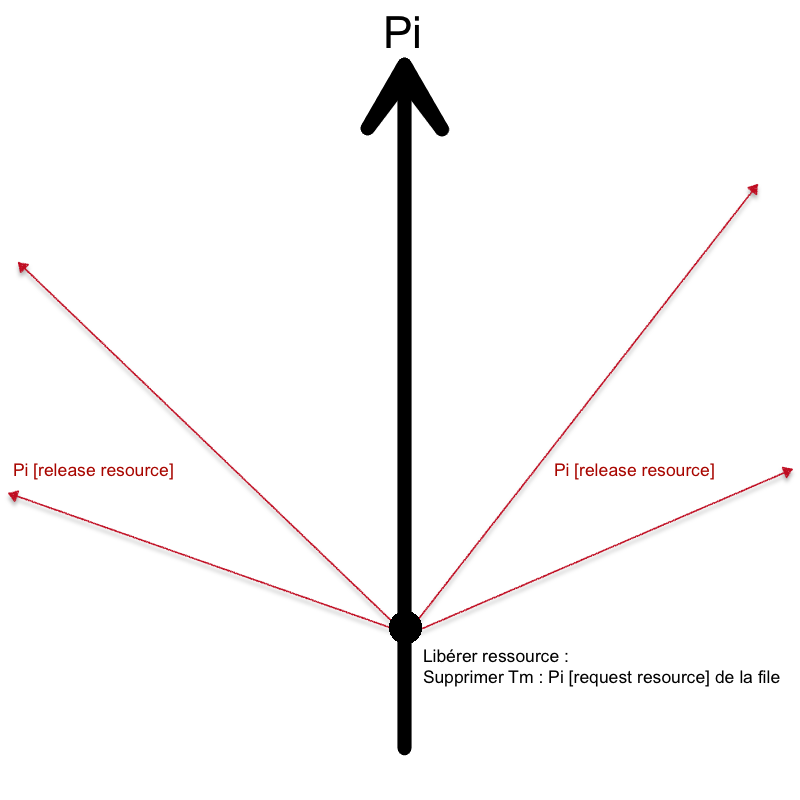
\includegraphics[scale=0.13]{process10.png}
		\end{column}
	\end{columns}
\end{frame}

\begin{frame}
\frametitle{Algorithme}
\begin{columns}
    	\begin{column}{.65\textwidth}
			Lorsque le processus $P_j$ reçoit un message contenant $P_i$[release resource], il supprime chaque requête $T_m : P_i$[request resource] de sa file de requête.
		\end{column}
		\begin{column}{.35\textwidth}
			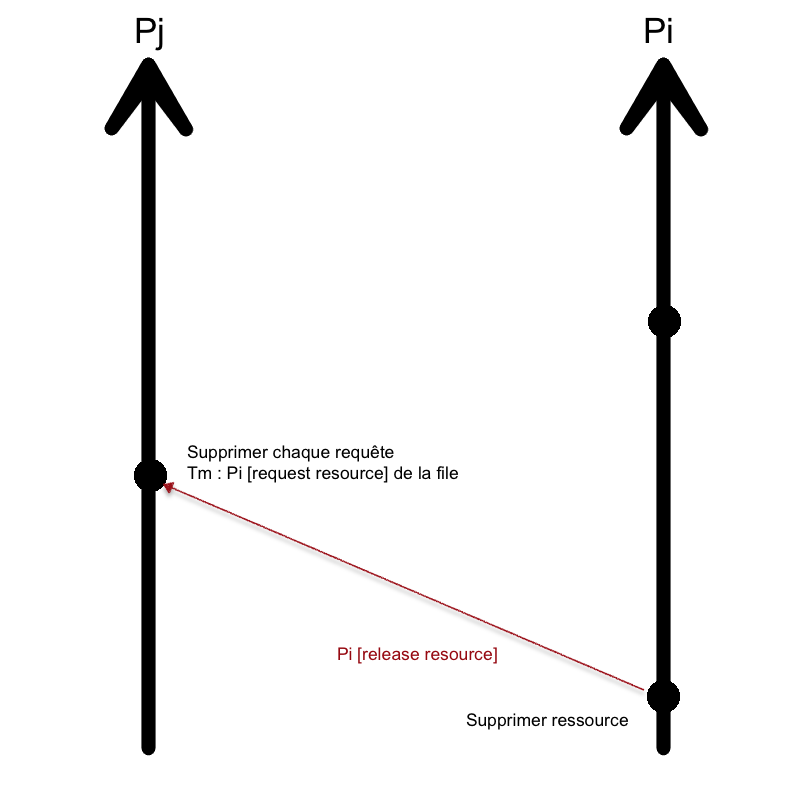
\includegraphics[scale=0.13]{process11.png}
		\end{column}
	\end{columns}
	Finalement, la ressource est accordée au processus $P_i$ lorsque
	\begin{itemize}
	\item Il y a un message contenant $T_m : P_i$[request resource] dans sa file de requête qui est ordonnée avant chaque autre requête dans sa file par la relation $\Rightarrow$.
	\item $P_i$ a reçu un message (ACK) de tous les autres processus qui est daté après $T_m$.
	\end{itemize}
	{\color{cyan} Chaque processus} suit ces règles indépendamment $\implies$ pas de processus de synchro et de stockage central.
\end{frame}

\begin{frame}
\frametitle{Généralisation}
\textbf{\color{cyan} But : }implémenter la synchronisation dans de tels systèmes distribués.\\
\begin{block}{Automate $SM(S, C, \delta)$}
\begin{itemize}
\item $S$ ensemble des états possibles. \\Un état $s$ correspond à une file de requêtes où la requête à la tête de la file est actuellement accordée.
\item $C$ ensemble des commandes possibles. \\Correspond aux commandes $P_i $ [request resource] et $P_i$ [release resource].
\item $\delta : S \times C \rightarrow S$ tel que $\forall s \in S, c \in C, \delta(s, c) = s'$ si il est possible d'exécuter la commande $c$ en $s$
\end{itemize}
\end{block}
\end{frame}

\begin{frame}
\frametitle{Simple Exemple}
\begin{figure}
	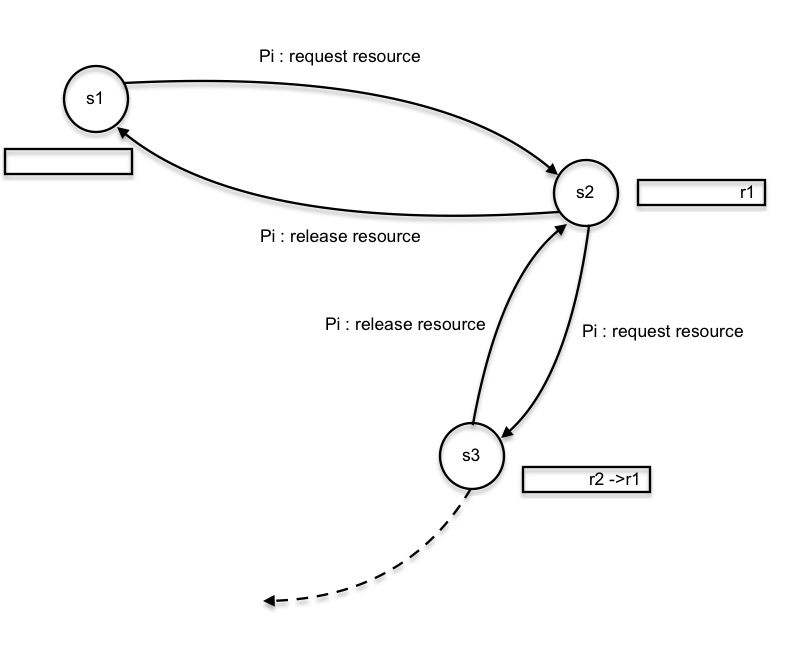
\includegraphics[scale=0.2]{state_machine.png}
\end{figure}
Chaque processus exécute indépendamment un tel automate. \\
En pratique, l'automate est plus complexe incluant des commandes avec des Timestamp $T_m$ et les commandes provenant des autres processus (ACK, request, release,...).
\end{frame}

\begin{frame}
\frametitle{Points faibles}
\begin{itemize}
\item L'algorithme nécessite la participation active de tous les autres processus
\item Un processus \textbf{doit} connaitre toutes les commandes issues des autres processus. 
\item L'échec d'un processus peut dérégler tout le système.
\item Sans \textbf{\color{cyan} temps physique}, il n'y a pas moyen de distinguer l'échec d'un processus d'un autre qui est juste en pause.
\end{itemize}
Cependant, le fait que l'algorithme classe les requêtes selon l'ordre total $\Rightarrow$ permet de détecter les comportements anormaux.
\end{frame}

% /!\ J'ai pas compris la suite Anomalous Behavior /!\

\section{Horloges Physiques}
\begin{frame}
\frametitle{Horloges Physiques : cas continu}
Soit $C_i(t)$, la lecture de l'horloge $C_i$ au temps physique $t$.
\begin{itemize}
\item On suppose que les horloges tournent en continu.
\item On passe des cas discrets au cas continus.
\item On suppose que $C_i(t)$ est \textit{dérivable},\\
	sauf pour les sauts discontinus où l'horloge est réinitialisée.
\item $\frac{\partial C_i(t)}{\partial t}$ représente le taux par rapport auquel $C_i(t)$ est synchronisé avec l'horloge physique au temps $t$.
\item Ce taux devrait être $\approx 1$.
\end{itemize}
\end{frame}

\begin{frame}
\frametitle{Propriétés}
\begin{block}{PC 1}
$\exists \kappa \ll 1$ tel que $\forall i, |\frac{\partial C_i(t)}{\partial t} - 1| < \kappa$
\end{block}
exemple : \textit{horloges à cristal $\kappa \leq 10^{-6}$}
Cette condition n'est pas assez forte : les horloges doivent être synchronisées c.à.d.
\[\forall i, j, t \ \ C_i(t) \approx C_j(t)\]
\begin{block}{PC 2}
$\exists \epsilon > 0, \forall i, j \ \ |C_i(t) - C_j(t)| < \epsilon$
\end{block}
$\kappa$ et $\epsilon$ doivent assurer d'éviter les anomalies.\\
\end{frame}

\begin{frame}
\frametitle{\'Eviter les comportements anormaux}
Soient $\mu \in \mathbb{R}^{> 0}$ , $a, b$ des évènements de deux processus distincts et le temps physique $t$.\\
\textbf{Si $a$ se produit en $t$ et que $b$ satisfait {\color{cyan}$a \rightarrow b$}, alors $b$ se produit en {\color{cyan}$t + \mu$.}}\\
exemple : Soient $sp$, le plus court chemin entre les processus et $c$, la vitesse de la lumière. On peut prendre $\mu = \frac{sp}{c}$
\begin{block}{Propriétés}
On suppose également que quand l'horloge est réinitialisée, elle est toujours remise en avant et jamais en arrière. Alors, pour éviter les comportements anormaux :
\[ C_i(t+\mu) - C_i(t) > (1 - \kappa)\mu\]
\[ C_i(t+\mu) - C_j(t) > 0 \text{ avec } \frac{\epsilon}{1-\kappa} \leq \mu \text{ (par PC 2)} \]
\end{block}
\end{frame}

\begin{frame}
\frametitle{\'Eviter les comportements anormaux}
\begin{block}{Propriétés}
On suppose également que quand l'horloge est réinitialisée, elle est toujours remise en avant et jamais en arrière. Alors, pour éviter les comportements anormaux :
\[ C_i(t+\mu) - C_i(t) > (1 - \kappa)\mu\]
\[ C_i(t+\mu) - C_j(t) > 0 \text{ avec } \frac{\epsilon}{1-\kappa} \leq \mu \text{ (par PC 2)} \]
\end{block}
\end{frame}

\begin{frame}
\frametitle{Délai d'envoi}
Soit $m$, un message envoyé au temps physique $t$ et reçu au temps $t'$.\\
{\color{cyan}$v_m = t' - t$} est le \textbf{\color{cyan}délai total} du message $m$.\\
Ce délai est non connu du processus qui reçoit $m$. On suppose par contre que tout processus recevant $m$ connait le\\ \textbf{\color{cyan} délai minimal de $m$ : } $0 \leq \mu_m \leq v_m$. \\
\textbf{\color{cyan} délai imprévisible de $m$ : }$\xi_m = v_m - \mu_m$
\end{frame}

\begin{frame}
\frametitle{Implémentation}

\end{frame}

\end{document}